\documentclass[smallcondensed]{svjour3}


%\documentclass[twoside]{article}


\usepackage{hyperref}
\usepackage{amssymb}
\usepackage{amsmath}
\usepackage{color}




\usepackage{mathabx}
\usepackage{tikz}
\usepackage{url}

\smartqed



\makeatletter
\newcommand{\labitem}[2]{%
\def\@itemlabel{\textbf{#1}}
\item
\def\@currentlabel{#1}\label{#2}}
\makeatother




\title{ The Sitnikov problem for several primary bodies configurations        }






\author{Gast\'on Beltritti   \and Fernando Mazzone   \and Martina Oviedo  }

\institute{G. Beltritti \at CONICET - Dpto. de Matem\'atica, Facultad de Ciencias Exactas Físico-Químicas y Naturales.
Universidad Nacional de R\'{i}o Cuarto
(5800) R\'{\i}o Cuarto, C\'ordoba, Argentina\\
\email{gbeltritti@exa.unrc.edu.ar}\\
F. Mazzone \at CONICET - Dpto. de Matem\'atica, Facultad de Ciencias Exactas Físico-Químicas y Naturales.
Universidad Nacional de R\'{i}o Cuarto
(5800) R\'{\i}o Cuarto, C\'ordoba, Argentina\\
\email{fmazzone@exa.unrc.edu.ar}\\
M. Oviedo \at
 CONICET - Instituto de Investigaciones Matem\'aticas ``Luis A. Santal\'o''.
 Facultad de Ciencias Exactas y Naturales-UBA.
 (C1428EGA) – C.A.B.A., Argentina.\\
\email{ moviedo@itba.edu.ar}
}



\newcommand{\rr}{\mathbb{R}}
\newcommand{\nn}{\mathbb{N}}



\begin{document}


\maketitle


\begin{abstract}
In this paper we address an $n+1$-body gravitational problem governed by the Newton's laws, where $n$ primary bodies orbit on a plane $\Pi$ and an additional massless particle moves on the perpendicular line to $\Pi$ passing through the center of mass of the primary bodies. We find a condition for the described configuration to be possible. The case that the primaries are in a rigid motion we classify all the motions of the massless particle. We study the situation when the massless particle has a periodic motion with the same minimal period than primary bodies. We show that this fact is related to the existence of \textcolor{red}{a} certain pyramidal central configuration.
\end{abstract}









\section{Introduction}
In this paper we study the following restricted  Newtonian $n+1$-body problem $P$ (see figure \ref{fig:conf_esp}):
\begin{itemize}
 \item[$P_1$] We have $n$ primary bodies of masses $m_1,\ldots,m_n$ and an additional massless particle.
 \item[$P_2$] The primary bodies are in a homographic motion (see \cite[Section 2.9]{JaumeLlibre276}). This motion is carried out in a plane $\Pi$.
 \item[$P_3$] The massless particle is moving  on the perpendicular line to $\Pi$ passing through the center of mass of the primary bodies.
\end{itemize}

\begin{figure}[h]
\begin{center}
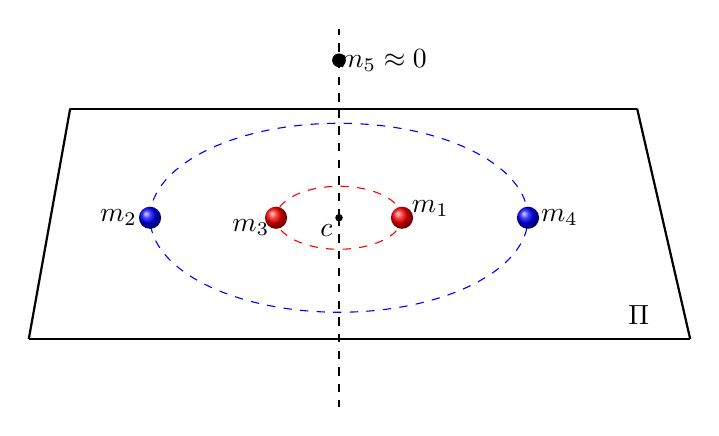
\begin{tikzpicture}[xscale=.8, yscale=.8]
				%Plano
				\draw[black,  line width=.8pt] (-6,0,-4.5)--(3,0,-4.5);
				\draw[black, line width=.8pt] (-3,0,5)--(7.5,0,5);
				\draw[black, line width=.8pt] (-3,0,5)--(-6,0,-4.5);
				\draw[black, line width=.8pt] (3,0,-4.5)--(7.5,0,5);
				%Elipses
				\draw[red,dashed] (0,0,0) ellipse (1cm and 0.5cm);
				\draw[blue,dashed] (0,0,0) ellipse (3cm and 1.5cm);
				%Cuerpos
					\shade[ball color=red]  (1,0) circle (5 pt);
					\node at (1.45,0.14) {$m_1$};
					\shade[ball color=red]  (-1,0) circle (5 pt);
					\node at (-1.4,-0.15) {$m_3$};

					\shade[ball color=blue]  (3,0) circle (5 pt);
					\node at (-3.5,0) {$m_2$};
					\shade[ball color=blue]  (-3,0)
					 circle (5 pt);
					\node at (3.5,0) {$m_4$};

					%eje z
        \draw[black, dashed, line width=.8pt] (0,0,0)--(0,3,0);
		\draw[black, dashed, line width=.8pt] (0,0,0)--(0,-3,0);
				% particula sin masa
		\draw[fill=black](0,2.5,0) circle (0.1 cm);
		\node at (0.7,2.5,0) {$m_5\approx 0$};
				%PI
				\node at (6.3,0,4) {$\Pi$};

				% CENTRO DE MASAS
				\draw[fill=black](0,0,0) circle (0.05 cm);
				\node at (-0.2,-0.2,0) {$c$};
\end{tikzpicture}\caption{Five-body problem with primaries in a collinear configuration}\label{fig:conf_esp}
\end{center}
\end{figure}


Problems like the one presented above have been extensively discussed in the literature. In \cite{sitnikov1960existence} K. Sitnikov considered the problem of two bodies in a Keplerian elliptic motion and a massless particle moving on the perpendicular line to the orbital plane passing
through the center of mass. Sitnikov obtained deep results about existence of solutions, for small $e>0$, with a chaotic behavior (see \cite[III(5)]{moser2016stable}). Periodic solutions for a Sitnikov configuration were considered in
\cite{corbera2000periodic,corbera2002symmetric,llibre2008families,pustyl1990certain}.


Generalized circular Sitnikov problems, i.e. when there are $n\geq 3$ primaries in a relative equilibrium motion,   were addressed more recently.
In \cite{soulis2008periodic} Soulis, Papadakis and Bountis studied existence, linear stability and bifurcations for a problem similar to $P$. They considered  a Lagrangian equilateral triangle configuration for the primary bodies, which were supposed to have the same mass $m_1=m_2=m_3$. In \cite{bountis2009stability} Papadakis and Bountis extended the results of \cite{soulis2008periodic} to $n$ primaries ($n\geq 3$) in a polygonal equal masses configuration. Later,  in \cite{pandey2013periodic}, Pandey and Ahmad generalized  the analysis started in \cite{soulis2008periodic} to the case with oblate primaries.
In \cite{li2013characterization} Li, Zhang and Zhao studied a special type of
restricted circular $n+1$-body problem  with equal masses for the primaries in a regular polygonal configuration. Periodic solutions for generalized Sitnikov problems with primaries performing  no rigid motions were studied in \cite{pustyl1990certain,rivera2013periodic}. We emphasize that in
\cite{bountis2009stability,li2013characterization,pandey2013periodic,pustyl1990certain,rivera2013periodic,soulis2008periodic} it is \textcolor{red}{assumed} that
the primary bodies are in the vertices of a regular polygon.
As far as we know, the first non-polygonal configuration of primary bodies was considered in \cite{marchesin2013spatial} where  Marchesin and Vidal studied the problem $P$ for a rigid motion  of primaries in a  rhomboidal configuration.
 In \cite{bakker2015separating} Bakker and Simmons studied scape regions for the massless particle in a  \textcolor{red}{similar problem} to $P$ where the primaries performe certain type of periodic orbits including non homographic motions.


In the present paper, after introducing preliminary facts in Section \ref{sec:pre},   we
obtain in Section \ref{sec:admisible.configuraciones} necessary and sufficient conditions on the configuration of primary bodies \textcolor{red}{in order}  the $z$-axis to be invariant for the flow associated to the motion equations of the massless particle. For this type of configurations, that we call \emph{\textcolor{red}{admissible}}, the Sitnikov problem has sense. \textcolor{red}{The conclusions of Section 3 are obtained basically by elementary linear algebra arguments. We consider that the main contribution of Section 3 is to expand the variety of problems of Sitnikov type.}  In Section \ref{sec:addmisibles}, \textcolor{red}{we find} all \textcolor{red}{admissible} configurations for $n\leq 4$ primaries. \textcolor{red}{The Perpendicular Bisector Theorem of Moeckel (see \cite{moeckel1990central}) is an important help to solve this question.} \textcolor{red}{In Section \ref{sec:mas-mot} we describe} all possible motions of the massless particle when the
primaries are in a relative equilibrium (or rigid) motion.  In this direction, we observe that only scape (both parabolic and hyperbolic) and periodic motions are possible.  \textcolor{red}{We also } give in Theorem \ref{thm:prop.periodos} a formula expressing the period of solutions  by means of integrals.  We prove in Corollary \ref{cor:sol.periodica.sist.completo} that the complete $n+1$-body system has  infinite quantity of periodic solutions. \textcolor{red}{We solve some problems raised in Section 5 by two alternative techniques: i) elementary arguments, by using energy conservation (\cite[Ch. 2]{A}) and ii) variational techniques inspired in \cite{li2013characterization,David-2004,zhao2015nonplanar}.} In Section  \ref{sec:sincro} we
discuss the
situation when the entire system has a solution with the same period as the motion of primaries. We call it \emph{synchronous solution}. Surprisingly, the existence of synchronous solutions is related to the existence of certain pyramidal central configurations (for the definition of this concept see \cite{fayccal1996classification,faycaltesis,ouyang2004pyramidal}). Finally, in the last section, we study certain non \textcolor{red}{admissible} configurations which provide some particular solutions of problem $P$.

In this paper we generalize and extend some \textcolor{red}{previously  obtained results. For example, the results in Section \ref{sec:mas-mot}, obtained for  admissible configurations},  generalize some results  in \cite{marchesin2013spatial} established for rhomboidal configurations. In Section \ref{sec:sincro} we prove that there exists synchronous solutions for primaries in a regular polygonal equal mass configuration if and only if $2\leq n\leq 472$. The \textcolor{red}{sufficiency} of this fact was established in \cite{li2013characterization}.


\section{Preliminaries}\label{sec:pre}

We start considering $n$  mass points, $n>2$, of masses $m_1,\ldots,m_n$ moving in a Euclidean 3-dimensional space according to Newton's laws of motion. We assume that $x_1(t),\ldots,x_n(t)$ are the coordinates of the bodies in some inertial Cartesian coordinate system.  We can suppose, without any loss of generality, that the center of mass   $C:=\sum_jm_jx_j/M$ ($M:=\sum_j m_j$) is fixed at the origin ($C=0$).

Initially we suppose that the bodies are in a \emph{planar homographic motion} on the plane $\Pi$ (see \cite{JaumeLlibre276}), where  $\Pi$ is the plane determined by the first two coordinates axes. Concretely,  we are assuming  that

\begin{equation}\label{eq:x_j=rtQtq_j}
 x_j(t)=r(t)Q(\theta (t))q_j,
\end{equation}
where
\[
 Q(\theta )=\begin{pmatrix}
           \cos(\theta ) & -\sin(\theta ) & 0\\
           \sin(\theta ) & \cos(\theta ) & 0\\
           0            &     0     &  1\\
          \end{pmatrix}
\]
and $q_j\in\Pi$, $j=1,\ldots,n$ are vectors in a planar \emph{central configuration} (CC) in $\Pi$. We recall the following definition of this concept (see \cite{JaumeLlibre276}).

\begin{definition}\label{def:CC}
Let $q=(q_1,\ldots,q_n)$ be  an n-tuple of positions in $\rr^3$ and let $m=(m_1,\ldots,m_n)$ be a vector of masses. We say that $(q,m)$ is a central configuration if
there exists $\lambda\in\rr$ such that
\begin{equation}\label{eq:def.CC}
\nabla_jU(q_1,\ldots,q_n)+\lambda m_jq_j=0,\quad j=1,\ldots,n,
\end{equation}
where
\begin{equation}\label{eq:potencial}
 U(q_1,\ldots,q_n)=\sum_{i<j}\frac{m_im_j}{r_{ij}},
\end{equation}
 $r_{ij}=|q_i-q_j|$ and $\nabla_j$ denotes the $3$-dimensional partial gradient with respect to $q_j$.
\end{definition}



From \cite[Eq. (2.16)]{JaumeLlibre276},  the functions $r(t)$ and $\theta (t)$ solve the two-dimensional Kepler problem in polar coordinates, which is 
\begin{equation}
 \begin{array}{rl}\label{eq:kepler.2.dim}
\ddot{r}(t)-r(t)\dot{\theta}(t)^2 & = -\frac{\lambda}{r(t)^2}\\
\frac{d }{dt}\left[ r(t)^2\dot{\theta}(t)\right] & =0.\\
\end{array}
\end{equation}
\textcolor{red}{It may be the case that the solutions of \eqref{eq:kepler.2.dim} are defined only on a proper subset of $\rr$. We denote  by $\mathcal{O}$ the domain of the solutions $r$ and $\theta$. In the particular case of \emph{rigid motion}, we have $\mathcal{O}=\rr$,  $r(t)\equiv 1$ and $\theta (t)=\sqrt{\lambda }t +\theta(0)$.} In this case the primary bodies perform a periodic motion with minimal period $T:=2\pi/\sqrt{\lambda }$.

Let $x_0(t)$ be the position of the massless particle.
According to the Newtonian equations of motion, $x_0$ satisfies
\begin{equation}\label{eq:newton}
 \ddot{x}_0=\sum_{i=1}^n\frac{m_i(x_i-x_0)}{|x_i-x_0|^3}=:f(t,x_0).
\end{equation}

In the previous equation, we assume that we know the positions of the primaries. Therefore, this equation plus  initial conditions  determine the position of the particle completely.


\section{\textcolor{red}{Admissible} configurations}\label{sec:admisible.configuraciones}
Henceforth, we denote by $L$ the coordinate $z$ axis.
\textcolor{red}{
 A necessary and sufficient condition for that $L$  be invariant under the  flow associated to the non autonomous system  \eqref{eq:newton} is  $f(t,L)\subset L$ for all $t\in\mathcal{O}$, i.e. $L$ is \emph{$f$-invariant} for every $t\in\mathcal{O}$. This fact follows by applying \cite[Th. 1]{Hai-1970} to the first order autonomous system
}
\[
\textcolor{red}{
 \left\{
  \begin{array}{cc}
   \frac{ds}{dt}&=1\\
   \frac{dx}{dt}&=v\\
   \frac{dv}{dt}&=f(s,x)\\
  \end{array}
 \right.}
\]
\textcolor{red}{which is equivalent to equation  \eqref{eq:newton}. In addition, the following observations must be taken into account: i) the autonomous vector field $F(s,x,v)=(1,v,f(s,x))$ satisfies $F(\mathcal{O}\times L\times L)\subset \mathcal{O}\times L\times L$ if and only if $f(t,L)\subset L$ for all $t\in\mathcal{O}$ and ii) if $A\subset \rr^d$ is a subspace,  $x\in A$ and $v\in\rr^d$ then $d(x+hv,A)/h\to 0$, when $h\to 0$ if and only if $v\in A$. In the last assertion $d$ denotes the distance function.}






\textcolor{red}{
\begin{definition}
We say that a
central configuration $(q,m)$ is \emph{admissible} if and only if
\begin{enumerate}
 \item  $q_i\neq 0$, for $i=1,\ldots,n$.
 \item For any $r>0$, if the set
\[F_r:=\{i:|q_i|=r\}\]
is non empty, then
\begin{equation}\label{eq:suma0}\sum_{i\in F_r}m_iq_i=0,\end{equation}
i.e. every maximal set of  bodies which are equidistant from origin has center of mass equal to $0$.
\end{enumerate}
\end{definition}
}

\textcolor{red}{\begin{remark}In the previous definition we introduce the condition $q_i\neq 0$  in order to avoid some collisions between the primaries and the particle.\end{remark}}

\begin{theorem}\label{thm:prim} $L$ is $f$-invariant for every \textcolor{red}{$t\in\mathcal{O}$} if and only if $(q,m)$ is \textcolor{red}{admissible}.
\end{theorem}

For the proof of the previous theorem we need the following result.


\begin{lemma}\label{lem:1} For $c>0$ we define the function $y_c(t):=(c+t)^{-3/2}$. If $0<t_1<t_2<\ldots<t_k$ then the functions $y_j(t):=y_{t_j}(t)$  are linearly independent on  each open interval   $I\subset \mathbb{R}^+$.
\end{lemma}
\begin{proof} It is sufficient to prove that the Wronskian

 \[W:=W(y_1,\ldots,y_k)(t)=\det\begin{pmatrix}
			      y_1 & \cdots & y_k\\
			      \frac{dy_1}{dt}&  \cdots & \frac{dy_k}{dt}\\
			      \vdots & \ddots & \vdots \\
			      \frac{d^{k-1}y_1}{dt^{k-1}}&  \cdots & \frac{d^{k-1}y_k}{dt^{k-1}}\\
                           \end{pmatrix}
\]
is not null on $I$.

Using induction, it is easy to show that
\begin{equation}\label{eq:der_ind}\frac{d^iy_c}{dt^i}=\beta_{i}y_{c}^{\frac{2i+3}{3}},\quad\hbox{for some }\beta_{i}\neq 0, \hbox{ and for all }i=1,\ldots.
\end{equation}
Fix any $t\in I$. Then, according to \eqref{eq:der_ind} and writing $\lambda_j:=(t+t_j)^{-1}$, we have

\[
\begin{split}
  W(t)&=\det
    \begin{pmatrix}
      \lambda_1^{3/2} & \lambda_2^{3/2} &\cdots & \lambda_k^{3/2} \\
      \beta_1\lambda_1^{5/2} &\beta_1 \lambda_2^{5/2} &\cdots &\beta_1 \lambda_k^{5/2}\\
      \vdots & \vdots &\ddots & \vdots\\
      \beta_{k-1}\lambda_1^{k+1/2} & \beta_{k-1}\lambda_2^{k+1/2} &\cdots & \beta_{k-1}\lambda_k^{k+1/2}
    \end{pmatrix}
  \\
  &= \beta_1\beta_2\cdots\beta_{k-1} \lambda_1^{3/2}\lambda_2^{3/2}\cdots \lambda_k^{3/2}
     \det \begin{pmatrix}
      1& 1 &\cdots & 1 \\
      \lambda_1 & \lambda_2 &\cdots & \lambda_k\\
      \vdots & \vdots &\ddots & \vdots\\
      \lambda_1^{k-1} & \lambda_2^{k-1} &\cdots & \lambda_k^{k-1}
    \end{pmatrix}
  \\
  &= \beta_1\beta_2\cdots\beta_{k-1} \lambda_1^{3/2}\lambda_2^{3/2}\cdots \lambda_k^{3/2}
  \prod_{1\leq i<j\leq n}(\lambda_j-\lambda_i)
,
\end{split}
\]
where the last equality follows from the well known Vandermonde determinant identity. Therefore, 
$W\neq 0$ if and only if $\lambda_i\neq\lambda_j$, $i\neq j$,
which in turn is equivalent to $t_i\neq t_j$, $i\neq j$.\qed
\end{proof}








\begin{proof}[Proof of Theorem \ref{thm:prim}]
The condition $f(t,L)\subset L$ for all $\textcolor{red}{t\in\mathcal{O}}$ is equivalent to
\begin{equation}\label{eq:f(L)cL-->sum=0}
 \sum_{i=1}^n\frac{m_ir(t)Q(\theta (t))q_i}{\left(r(t)^2|q_i|^2+z^2\right)^{3/2}}=0\in\rr^2,
\end{equation}
for every $\textcolor{red}{t\in\mathcal{O}}$ and $z\in \rr$.

Let $D=\{|q_i|: i=1,\ldots,n\}$.  Suppose that $D=\{s_1,\ldots,s_k\}$, with $s_i\neq s_j$ for $i\neq j$.  Therefore $\{1,\ldots,n\}=F_{s_1}\cup \cdots\cup F_{s_k}$. Then, multiplying equation \eqref{eq:f(L)cL-->sum=0} by $r(t)^2Q^{-1}(\theta(t))$  and writing $\zeta=(z/r(t))^2$ we have that \eqref{eq:f(L)cL-->sum=0} is equivalent to


\[\sum_{j=1}^k\left\{\frac{1}{(s_j^{2}+\zeta)^{3/2}}\sum_{i\in F_{s_j}}m_iq_i\right\}=0.\]
According to Lemma \ref{lem:1}, the last equation is equivalent to \eqref{eq:suma0}. \qed
\end{proof}


\section{\textcolor{red}{Admissible}  configurations for $n\leq 4$}\label{sec:addmisibles}


In this section, we find all \textcolor{red}{admissible}  configurations with $n\leq 4$.    Since the center of mass is an excluded position, an \textcolor{red}{admissible} configuration satisfies
\textcolor{red}{
\begin{equation}\label{F_r.no.vac-->CF_r.geq2}
 \# F_r\neq 1.
\end{equation}
}


It is a trivial fact that  two point masses $m_1$ and $m_2$ configuration is \textcolor{red}{admissible} if and only if $m_1=m_2$.


From \eqref{F_r.no.vac-->CF_r.geq2}, a $3$-body \textcolor{red}{admissible}  configuration consists of equidistant  bodies from the origin. Therefore, it must  be the Lagrangian equilateral triangle. Now, by equation \eqref{eq:suma0} and an elementary geometrical reasoning,   we have  $m_1=m_2=m_3$.



The case $n=4$ is more interesting. We include Definition \ref{def:bis.per} and Theorem \ref{thm:bisector.moeckel}, which were introduced  for the first time in  \cite{moeckel1990central}, for the reader's convenience.

\begin{definition}\label{def:bis.per}
Let $q$ be a planar configuration. For each pair, $i$, $j$, the line
containing $q_i$ and $q_j$ together with its perpendicular bisector form axes which
divide the plane into four quadrants. The union of the first and third quadrants
is an hourglass shaped region which will be called a `cone'; similarly,
the second and fourth quadrants together form another cone. The phrase `open
cone' refers to a cone minus the axes.
\end{definition}

\begin{theorem}[Perpendicular Bisector Theorem]\label{thm:bisector.moeckel}
Let $(q,m)$ be a planar central configuration and let
$q_i$ and $q_j$ be any two of its points. Then if one of the two open cones determined
by the line through $q_i$ and $q_j$ and its perpendicular bisector contains points of
the configuration, so does the other one.
\end{theorem}

Next, we characterize all the $4$-body \textcolor{red}{admissible}  configurations.

\begin{theorem}\label{thm:caracterizacion4}
Let $(q,m)$ be a 4-body central configuration. Then $(q,m)$ is  \textcolor{red}{admissible} if and only if, \textcolor{red}{$q_i\neq 0$} and  for a suitable enumeration  of bodies,   $q_1=-q_3$, $q_2=-q_4$, $m_1=m_3$,  $m_2=m_4$, and  $(q,m)$ is of some of the following mutually exclusive types:
\begin{description}
\item[CCcl.]   collinear,
\item[CCr.]  a rhombus with $r_{13}<r_{24}$ and $m_1>m_2$,
\item[CCs.]  a square with four equal masses.
\end{description}
\end{theorem}




\begin{remark} In \cite{shoaib2011collinear}  central configurations of type CCcl were studied; while,  CCr configurations were treated in \cite{long2002four} and \cite{perez2007convex}.

\end{remark}



\begin{proof}
From \eqref{F_r.no.vac-->CF_r.geq2} we have to consider two cases.

\emph{Case 1.}  $m_1\geq m_2$, $|q_1|\neq|q_2|$, $|q_1|=|q_3|$ and $|q_2|=|q_4|$. Now \eqref{eq:suma0} implies that
 $m_1=m_3$, $m_2=m_4$, $q_1=-q_3$ and $q_2=-q_4$.  We divide the plane into two open cones $C_i$, $i=1,2$, by means of  the line $P$ joining $q_1$  and $q_3$ together with its perpendicular bisector $M$.  From Theorem \ref{thm:bisector.moeckel}, if  $q_2$  is in $C_1$, then  $q_4$ is in $C_2$, and vice versa. This is a contradiction with the fact that $q_2=-q_4$. Then $q_2,q_4\in P$ or $q_2,q_4\in M$, i.e. $q$ is collinear or a rhombus with equal masses in opposite vertices. In the first case, $(q,m)$ is of  CCcl type. In the second case, if $m_1>m_2$,   was proved in \cite[Eqs. $(3.44)$ and $(3.45)$]{long2002four} that $r_{13}<r_{24}$. Hence $(q,m)$ is of  CCr type. From \cite[Corollary 2]{perez2007convex} if $m_1=m_2$ then the configuration is a square which is a contradiction with the fact that $|q_1|\neq|q_2|$.

\emph{Case 2.} $|q_1|=|q_2|=|q_3|=|q_4|$. In this situation,   in \cite{hampton2005co} it was proved that the configuration is the equal mass square.\qed
\end{proof}

\section{Massless particle motion}\label{sec:mas-mot}

In this section and in Section \ref{sec:sincro},  we will suppose that the primary bodies are in a $T$-periodic rigid motion associated to an \textcolor{red}{admissible}  CC $(q,m)$, i.e  $r(t)\equiv 1$ and according to remark \textcolor{red}{that follows} equation \eqref{eq:kepler.2.dim}, $\theta (t)=\sqrt{\lambda}t$  (w.l.o.g  we  assume that $\theta(0)=0$). \textcolor{red}{To} the particle, we suppose that it is moving on $L$, i.e. $x_0(t)=(0,0,z(t))$. From Theorem \ref{thm:prim}, $x_0$ is solution of \eqref{eq:newton}, if and only if $z(t)$ is solution of the autonomous equation



\begin{equation}\label{eq:eq_new_red}
 \ddot{z}=-\sum_{i=1}^n\frac{m_iz}{(s_i^2+z^2)^{3/2}},
\end{equation}
where $s_i=|q_i|$.

We will analyze all possible motions for the massless particle $x_0$. In particular, we will see that every motion is either periodic or a scape trajectory. We will find that there exist $T_0$-periodic solutions for all $T_0$ on an interval  $(\sigma(q,m),+\infty)$. This fact implies that there exists an infinity quantity of periodic solutions for the entire $n+1$-body system.





The second order equation \eqref{eq:eq_new_red} is conservative, therefore solutions conserve the energy
\begin{equation}\label{eq:conser.energ}
E(z,v):=\frac{|v|^2}{2}-\sum_{i=1}^{n} \frac{m_i}{\left(s_i^2+z^2\right)^{\frac12}},
\end{equation}
i.e. $E(z(t),\dot{z}(t))$ is constant.



Following \cite{VladimirI.Arnold229} (see also \cite{marchesin2013spatial})  we introduce the next concepts.
\textcolor{red}{
\begin{definition}[Chazy, 1922]
 Let  $z(t)$  be a solution of \eqref{eq:eq_new_red} such that $\lim\limits_{t\to\infty}z(t)=\infty$. Then $z(t)$ is called:
 \begin{itemize}
  \item   hyperbolic when there exists $\lim\limits_{t\to\infty}\dot{z}(t)$ and it is not null,
  \item  parabolic if $\lim\limits_{t\to\infty}\dot{z}(t)=0$.
 \end{itemize}
\end{definition}
}





The following theorem characterizes all the possible motions for the massless particle.

\begin{theorem}\label{thm:prin_ine} We assume that $(q,m)$ is an \textcolor{red}{admissible}  configuration and the primaries are in a rigid motion. Every solution of \eqref{eq:eq_new_red} is of some of the following types:
\begin{enumerate}
\item\label{1} Hyperbolic, when $E>0$,
\item\label{2} Parabolic, when $E=0$,
\item\label{3} Periodic, when $E_{min}:=-\sum_{i=1}^{n}\frac{m_i}{s_i}<E<0$.
\item\label{4} Equilibrium solution when $E=E_{min}$.
\end{enumerate}
\end{theorem}

\begin{proof}
We follow a standard argument for Hamiltonian systems (see \cite{A}).

We consider the level sets $S(E)=\{(z,v):E(z,v)=E\}$ on the phase space $(z,v)$. An elementary analysis shows that
\begin{itemize}
 \item If $E\geq 0$ then $S(E)$ is the union of two bounded graphs. They are symmetric with respect to $z$-axis, each of which is contained  in some semiplane $v> 0$ or $v<0$. The $v$-positive branch is the graph of a function $v(E,z)$, which  is decreasing with respect to $|z|$. Moreover, $\lim\limits_{|z|\to \infty}v(E,z)=\sqrt{2E}$.

 \item For every $E\geq E_{min}$, the energy curve $S(E)$ cuts the $v$-axis at the value $\pm(2E+2\sum_{i=1}^n m_is_i^{-1})^{\frac12}$.

 \item If $E_{min}<E<0$ then $S(E)$ is a simple closed curve symmetric with respect to $z$ and $v$ axes.

 \item  \textcolor{red}{An energy curve cuts the $z$-axis, only in the case that $E<0$, at the point $\pm z_{E}$,  where $z_E$ is the only positive solution of $-\sum_{i=1}^n m_i (s_i^2+z_{E}^2)^{-\frac12}=E$.}
\end{itemize}

In Figure  \ref{fig:conf_esp}, we show the phase portrait for a rhomboidal configuration with masses $m_1=m_3=1$ and $m_2=m_4=0.5$.

The function $\varphi(t)=(z(t),\dot{z}(t))$ solves the system $\dot{\varphi}(t)=F(\varphi(t))$, where \linebreak $F(z,v)=(v,-\sum_{i=1}^{n}m_iz (s_i^2+z^2)^{-3/2})$. \textcolor{red}{It is easy to show that the vector field $F$ has a bounded Jacobian  $D F$. Therefore $F(z,v)$ is a global Lipschitz function on $\rr^2$. This fact and \cite[Th. B.1]{betounes2009differential} imply that the trajectories $t\mapsto (z(t),\dot{z}(t))$ are defined for every time. On the other hand, since $\dot{z}=v$, the motion along trajectories is in clockwise direction. The only fixed point of $F$ is $(z,v)=(0,0)$.  Therefore, the level surfaces $S(E)$, with $E\neq E_{min}$, do not contain stationary points. Then the $\lim_{t\to\infty}\varphi(t)$ does not exists.  As consequence the map $t\mapsto \varphi(t)$    fills completely one connected component of its corresponding   energy curve.}

We observe that any solution $z$ crosses the $v$-axis. On the other hand, if $E\geq 0$ and $v(E,0)>0$ ($v(E,0)<0$) then $z(t)$ is increasing (decreasing) with respect to $t$. If $z(t)$ remained bounded when $t\to +\infty$, then there would be the limit $\zeta_{\infty}:=\lim\limits_{t\to\infty}z(t)$. This would imply  that $(\zeta_{\infty},0)$ would be a fixed point of $F$, which is a contradiction.  As a consequence, if $E\geq 0$ then $|z(t)|\to \infty$ when $t\to  +\infty$. Moreover $\lim\limits_{t\to +\infty}\dot{z}(t)=\pm\sqrt{2E}$.  From this fact, we conclude that the trajectory is hyperbolic when $E>0$ and it is parabolic in the case that $E=0$.

In the case that $E_{min}<E<0$, we have that the trajectory is contained in a closed curve; therefore, it is a periodic orbit.

Finally, if $E=E_{min}$  we clearly have that $z(t)\equiv 0$.
\begin{figure}[h]
\begin{center}
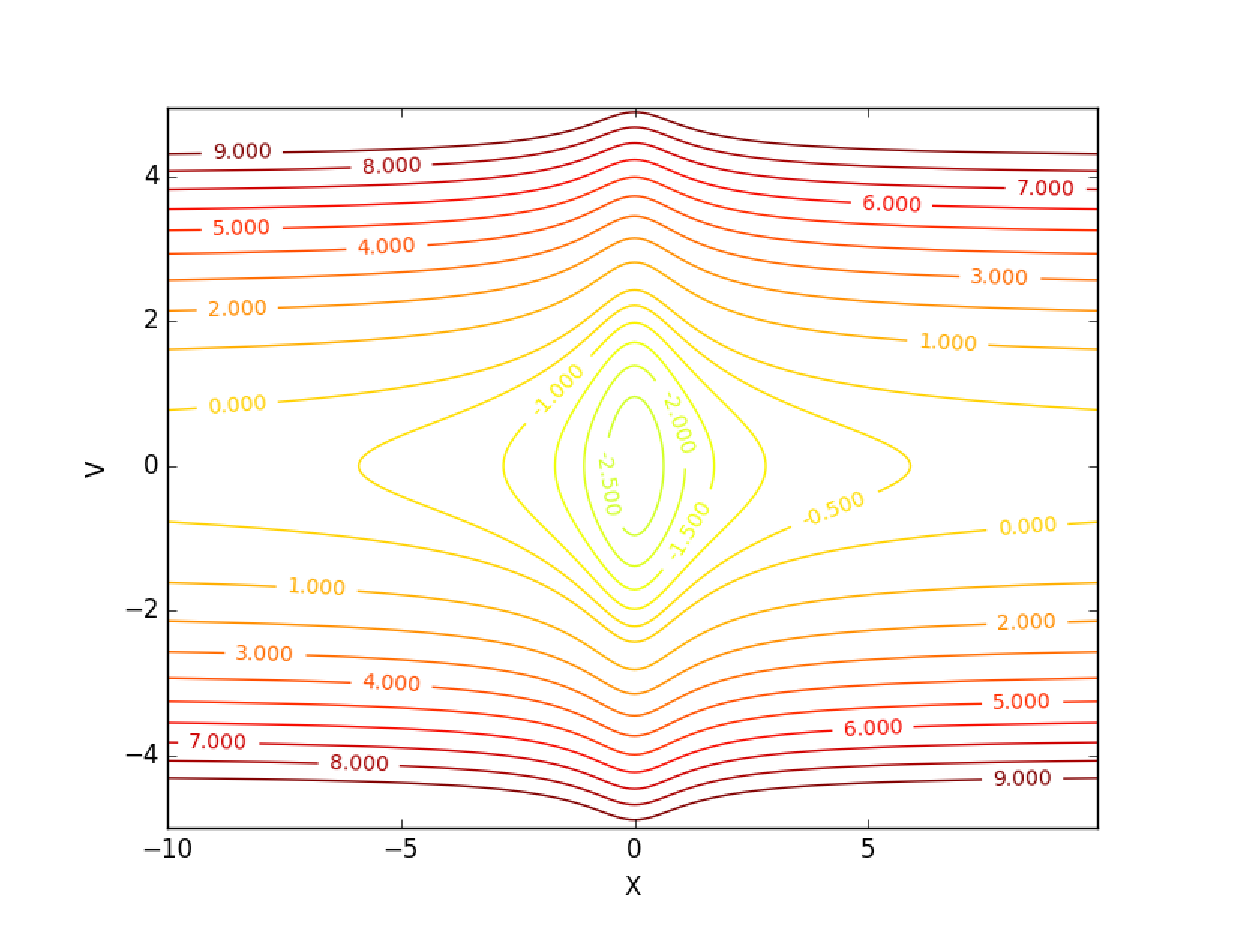
\includegraphics[scale=0.3]{figure_1.eps}
\caption{Energy level for a rhomboidal configuration with masses $m_1=m_3=1$ and $m_2=m_4=0.5$.}\label{fig:energy}
\end{center}
\end{figure}
\qed\end{proof}

\begin{theorem}\label{thm:prop.periodos}
We denote by $T_0(E)$ the minimal period for a solution of \eqref{eq:eq_new_red} with $E_{min}<E<0$. Then
\begin{enumerate}
 \item\label{it:T0.formula} 
 \begin{equation}\label{eq:form.T0E-periodo}
 T_0(E)=2^{3/2}\int_{0}^{z_E} \left(E+\sum_{i=1}^n m_i (s_i^2+z^2)^{-\frac12}\right)^{-\frac12} dz,
 \end{equation}
 where $z_E$ is the only positive solution of $-\sum_{i=1}^n m_i (s_i^2+z_{E}^2)^{-\frac12}=E$ ,
 \item\label{it:T0.creciente} $T_0(E)$ is an increasing function.
 \item\label{it:T0.rango} $T_0\left((E_{min},0)\right)=(T_{min},+\infty)$, where  $T_{min}=2\pi\left(\sum_{i=1}^n\frac{m_i}{s_i^3} \right)^{-1/2}$.

 \end{enumerate}
\end{theorem}

\begin{proof}
Let $E_{min}<E<0$ and let $z(t)$ be the only solution with $z(0)=0$, $\dot{z}(0)>0$ and energy equals to $E$. Therefore $z(t)$ is $T_0(E)$-periodic. As a consequence of the symmetries of the equation, we have that $z(T_0(E)/4)=z_E$. Then, taking account of \eqref{eq:conser.energ}, we have 
\begin{equation*}
 \begin{split}
  \frac{T_0}{4}&=\frac{1}{\sqrt{2}}\int_0^{T_0/4}\left(E+\sum_{i=1}^n m_i (s_i^2+z^2)^{-\frac12}\right)^{-\frac12} \dot{z} dt\\
  &=\frac{1}{\sqrt{2}}\int_{0}^{z_E} \left(E+\sum_{i=1}^n m_i (s_i^2+z^2)^{-\frac12}\right)^{-\frac12} dz,
 \end{split}
\end{equation*}
and we have proved item \textit{1}. In order to prove item \textit{2}, we note that
\begin{equation*}
 \begin{split}
  2^{-3/2}T_0(E)
  &=
    \int_0^{z_E}\left(\sum_{i=1}^n m_i \left((s_i^2+z^2)^{-\frac12}-(s_i^2+z_E^2)^{-\frac12}\right)\right)^{-\frac12}dz\\
  &=\int_0^{z_E} \left(z_E^2-z^2\right)^{-\frac12} f(z,z_E)dz\\
  &=\int_0^1 \left(1-u^2\right)^{-\frac12} f(z_Eu,z_E)du,
 \end{split}
 \end{equation*}
where \[f(z,z_E)=\left(\sum_{i=1}^n m_i \left\{(s_i^2+z^2)(s_i^2+z_E^2)\right\}^{-\frac12} \left\{(s_i^2+z^2)^{\frac12}+(s_i^2+z_E^2)^{\frac12} \right\}^{-1}\right)^{-\frac12}.\]
We point out that $f(z_Eu,z_E)$ is an increasing function with respect to $z_E$ for $u\in [0,1]$ fix. This assertion implies item \ref{it:T0.creciente}.

On the other hand,
\begin{equation*}
 \lim\limits_{z_E \to 0}f(z_Eu,z_E)=\left(\sum_{i=1}^{n} \frac{m_i}{2s_i^3}\right)^{-\frac12} \quad \text{and}\quad  \lim\limits_{z_E \to +\infty}f(z_Eu,z_E)=+\infty.
\end{equation*}
Thus, from the Dominated Convergence Theorem and Monotone Convergence Theorem, we have 
\[\lim\limits_{E\to E_{min}}T_0=\lim\limits_{z_E\to 0}T_0=2\pi\left(\sum_{i=1}^{n} \frac{m_i}{s_i^3}\right)^{-\frac12}\quad \text{and}\quad \lim\limits_{E\to 0}T_0=\lim\limits_{z_E\to +\infty}T_0=+\infty.\]
Finally,  since $T_0=T_0(z_E)$ is continuous and increasing with respect to $z_E$, we conclude the statement of item \ref{it:T0.rango}.
\qed\end{proof}

\begin{remark}
 It is possible to use the classical theory of Hamiltonian systems (see \cite{A}) to derive the formula \eqref{eq:form.T0E-periodo} (see \cite{acinas2014estimates} for this approach in a related problem).
\end{remark}



\begin{remark}
Let us show a second proof of item \ref{it:T0.rango} of Theorem \ref{thm:prop.periodos}.

The inequality $T_0>T_{min}$ is a consequence of comparison Sturm's theorem applied to equations  $\ddot{z}+h(z)z=0$, where $h(z)=\sum_{i=1}^{n} m_i \left(s_i^2 +z^2\right)^{-3/2}$, and $\ddot{z}+\left(\sum_{i=1}^{n} m_i s_i^{-3}\right)z=0$. This proves that $T_0\left((E_{min},0)\right)\subset(T_{min},+\infty)$.

For the reverse inclusion,  we  follow arguments of \cite{zhao2015nonplanar} and \cite{li2013characterization} based on variational principles.


Let $T_0>T_{min}$. We consider the action integral
\[\mathcal{I}(z)=\int_0^{T_0}\frac12|\dot{z}|^2+\sum_{i=1}^n\frac{m_i}{\sqrt{s_i^2+z^2}}dt,\]

Then $T_0$-periodic solutions of \eqref{eq:eq_new_red} are critical points of $\mathcal{I}$ in the space $H^1(\mathbb{T},\rr)$ of the functions which are  absolutely continuous, $T_0$-periodic with $\dot{z}\in L^2(\mathbb{T},\rr)$ and being $\mathbb{T}=\rr/T_0\mathbb{Z}$ (see \cite[Cor. 1.1]{Mawhin2010}). We prove the existence of critical points by means of the direct method of calculus of variations, i.e. we will prove that $\mathcal{I}$ has a minimum.  The functional $\mathcal{I}$ is not coercive in $H^1(\mathbb{T},\rr)$.  This deficiency is overcome with symmetry techniques (see \cite{David-2004}). The group $\mathbb{Z}_2$ acts on $H^1(\mathbb{T},\rr)$ according to the following assignments $(\bar{0}\cdot z)(t)=z(t)$ and $(\bar{1}\cdot z)(t)=-z(t+\frac{T_0}{2})$. The symmetry involved in previous definition is called \emph{Italian Symmetry}. The functional $\mathcal{I}$ is $\mathbb{Z}_2$-invariant, i.e. $\mathcal{I}(g\cdot z)=\mathcal{I}(z)$. We define the space of all $\mathbb{Z}_
2$-symmetric functions
\[\Lambda(\mathbb{T},\mathbb{R}):
=\left\{ z\in H^1(\mathbb{T},\rr) | \forall g\in \mathbb{Z}_2 : z=g\cdot z \right\}.\]
The functional $\mathcal{I}$ restricted to $\Lambda$  is coercive. This fact follows from an obvious adaptation of Proposition 4.1 of \cite{David-2004}. We note that $F(z):=\sum_{i=1}^nm_i(s_i^2+z^2)^{-\frac{1}{2}}$ satisfies the condition $(A)$ in \cite[p. 12]{Mawhin2010}, then $\mathcal{I}$  is continuously differentiable and weakly lower semicontinuous on $H^1(\mathbb{T},\rr)$ (see \cite[p. 13]{Mawhin2010}). Therefore $\mathcal{I}$ has a minimum $z_0$ in $\Lambda(\mathbb{T},\mathbb{R})$. Then by the Palais' principle of symmetric criticality,  $z_0$ is a critical point of $\mathcal{I}$ in $H^1(\mathbb{T},\rr)$ (see \cite{David-2004} and \cite{RichardPalais274}).

We use the second variation $\delta^2 \mathcal{I}$ in order to show  that $z_0\nequiv 0$. It is well known (see \cite[Th. 1.3.1]{jost1998calculus}) that if $z_0$ is a minimum of $\mathcal{I}$ on $H^1(\mathbb{T},\rr)$  then $\delta^2 \mathcal{I} (z_0,\varphi)\geq 0$ for all $\varphi\in H^1(\mathbb{T},\rr)$. In our case,
\[\delta^2\mathcal{I}(0,\varphi)=\int_0^{T_0} |\dot{\varphi}|^2-\sum_{i=1}^{n}\frac{m_i}{s_i^3}\varphi^2 dt,\]
(see \cite[Eq. 1.3.6]{jost1998calculus}). In particular, if $\varphi(t)=\sin (2\pi t/T_0)$ it follows from $T_0>T_{min}$  that
\begin{equation}\label{eq:form.delta2}
 \delta^2 \mathcal{I} (0,\varphi)=\left( \frac{4\pi^2}{T_0^2}-\sum_{i=1}^{n}\frac{m_i}{s_i^3} \right)\frac{T_0}{2}<0.
\end{equation}
It is sufficient  to guarantee that $z_0\equiv 0$ is not a minimum.\qed


This second proof, unlike the first one, does not prove that $T_0$ is the minimum period \textcolor{red}{of} $z_0$. It could happen that $z_0$ had period $T_0/m$, with natural $m\in\mathbb{N}$. Because of Italian symmetry this $m$ should be odd.
\end{remark}






\begin{corollary}\label{cor:sol.periodica.sist.completo}
The complete $n+1$-body system has an infinity quantity of periodic solutions.
\end{corollary}
\begin{proof} We recall that $T$ denotes minimal period of the primaries.
Let $l/m$  be a positive rational number with $Tl/m>T_{min}$. Then, there exists a solution of the entire system with period $lT$.
\qed\end{proof}





\section{Synchronous solutions and pyramidal CC}\label{sec:sincro}



If the equation \eqref{eq:eq_new_red} has a $T$-periodic solution,  we say that the solution is \emph{synchronous}. \textcolor{red}{In \cite{li2013characterization} the problem of existence of synchronous solutions for $n$ equal mass primary bodies in a regular polygon configuration  was studied.}

In this section we establish a relation between the existence of synchronous solutions and the concept of pyramidal central configuration (see \cite{fayccal1996classification,faycaltesis,ouyang2004pyramidal}).

\begin{definition}
A central configuration of $n+1$ mass point $q_0,\ldots,q_{n}$ in $\rr^{3}$  is called a pyramidal central configuration (PCC) if and only if $n$ points, we say $q_1,\ldots,q_n$, are in some plane $\Pi$ and $q_{0}\notin \Pi$.
\end{definition}

The following lemma was proved in \cite{ouyang2004pyramidal} (see also \cite{faycaltesis}).
\begin{lemma}[\cite{ouyang2004pyramidal}, Lemma 2.1]\label{lem:PCC}
 Let $q_0,\ldots,q_{n}$ be a PCC such that $m_{0}$ is off the plane containing $m_1,\ldots,m_n$. If $m_{0}>0$ then $m_{0}$ is equidistant from $m_1,\ldots,m_n$.
\end{lemma}

We remark that the condition $m_{0}>0$ is important in the previous lemma. \textcolor{red}{In the examples below, we will show  two PCC} with $m_{0}=0$ which do not satisfy the conclusion of  Lemma \ref{lem:PCC}.



\begin{proposition}\label{cor:sol.sincronica}
We assume that $q=q_1,\ldots,q_n$ is an \textcolor{red}{admissible}   configuration and that the primaries are in a rigid motion. Then, there is a synchronous solution if and only if there exists $c\in \rr$ such that the points $(0,0,c),q_1,\ldots,q_{n}$ associated to the masses $0,m_1,\ldots,m_{n}$ form a PCC.
\end{proposition}

\begin{proof}
We start assuming that there exist a synchronous solution. As a consequence of the Theorem \ref{thm:prop.periodos}(\ref{it:T0.rango}) and the fact that $T^2=4\pi^2/\lambda$, we get

 \begin{equation}\label{eq:lamdbda<suma.si3}
\lambda<\sum_{i=1}^n\frac{m_i}{s_i^3}.
 \end{equation}
 Since $\sum_{i=1}^{n}m_i\left(s_i^2+c^2\right)^{-3/2}\to 0$, when $c\to +\infty$, there exists $c\in \rr$ such that
 $ \sum_{i=1}^{n}m_i\left(s_i^2+c^2\right)^{-3/2}=\lambda$. Therefore
 \begin{equation}\label{eq:cond.CC1}
  -\sum_{i=1}^{n}\frac{m_i c}{\left(s_i^2+c^2\right)^{3/2}}=-\lambda c.
 \end{equation}
As $q_1,\ldots,q_n$ is an \textcolor{red}{admissible} configuration, then
\begin{equation}\label{eq:cond.CC2}
   \sum_{i=1}^{n}\frac{m_i q_i}{\left(s_i^2+c^2\right)^{3/2}}= (0,0).
\end{equation}
The equations \eqref{eq:cond.CC1}, \eqref{eq:cond.CC2}  and the fact that $q_1,\ldots,q_n$ is a CC with constant $\lambda$, complete the proof.
The proof of the reciprocal statement follows in a direct way.
\qed\end{proof}

\begin{corollary}
We assume that $(q,m)$ is an \textcolor{red}{admissible}  configuration and  the primaries are in a rigid motion. Then, there is a synchronous solution if and only if
 \begin{equation}\label{eq:ine_prin}
 \sum_{i<j}\frac{m_im_j}{r_{ij}}<\left(\sum_{i=1}^n\frac{m_i}{s_i^3}\right)\left(\sum_{i=1}^nm_is_i^2\right).
\end{equation}
\end{corollary}

\begin{proof}
The result is a consequence of \eqref{eq:lamdbda<suma.si3} and the fact that $T^2=4\pi^2 \sum_{i=1}^{n}m_is_i^2/U$   (see \cite[p. 109]{JaumeLlibre276}).
\qed\end{proof}


\begin{remark}\label{com:sincronicas}

Let $(q,m)$  be an  \textcolor{red}{admissible}  CC  with constant $\lambda>0$ satisfying \eqref{eq:ine_prin} and let $r,\mu$ be positive numbers. Then  $(rq,\mu m)$ is a CC with constant $\lambda \mu r^3$, and \eqref{eq:ine_prin} remains unchanged. In virtue of previous observation, we can assume that any  length and any mass take any  desired value. The equation \eqref{eq:eq_new_red} has a synchronous solution if and only if the same equation with $(rq,\mu m)$ instead of $(q,m)$ has a synchronous solution.

\end{remark}





The sufficiency of the condition $n\leq 472$ in the following corollary  was proved in \cite{li2013characterization}.

\begin{corollary}\label{cor:nleq472}
We suppose that $(q,m)$ is the equal masses regular polygon configuration  (this is an \textcolor{red}{admissible} CC). Then, there exists a synchronous solution if and only if $2\leq n\leq 472$.
\end{corollary}

\begin{proof}
In this case $s_1=s_2=\cdots=s_n=:r$ and $m_1=m_2=\cdots=m_n=:M$. Then, from the law of cosines, we obtain
\[
 \sum_{i<j}\frac{m_im_j}{r_{ij}}=\frac{nM^2}{4r}\sum_{j=1}^{n-1}\frac{1}{\sin\left(\frac{j\pi}{n}\right)}.
\]
Therefore, the condition \eqref{eq:ine_prin} is equivalent to

\begin{equation}\label{eq:ine_prin_LShShao}
  \frac1n\sum_{j=1}^{n-1}\frac{1}{\sin\left(\frac{j\pi}{n}\right)}<4.
\end{equation}

This inequality was also derived by Li, J. et al. in \cite{li2013characterization}, where the authors proved (performing computer calculations) that inequality \eqref{eq:ine_prin_LShShao} holds true for $2\leq n\leq 472$. Let us prove that any other $n$ does not satisfy \eqref{eq:ine_prin_LShShao}.


Using that $1/\sin (x)$ is a convex function on $[0,\pi]$ and the composite trapezoid rule (see \cite{kincaid1991numerical}), we have 
\[
\begin{split}
 \int_{\frac{\pi}{n}}^{\frac{n-1}{n}\pi}\frac{1}{\sin (x)}dx&\leq \frac{\pi}{2n}\left\{ \frac{1}{\sin(\frac{\pi}{n})} + \frac{1}{\sin(\frac{n-1}{n}\pi)} +2\sum_{j=2}^{n-2}\frac{1}{\sin(j\frac{\pi}{n})} \right\}\\
 &=\frac{\pi}{n}\sum_{j=1}^{n-2}\frac{1}{\sin(j\frac{\pi}{n})}.
\end{split}
\]
Hence
\[
\begin{split}
 \frac1n \sum_{j=1}^{n-1}\frac{1}{\sin\left(\frac{j\pi}{n}\right)}&\geq \frac{1}{\pi}\int_{\frac{\pi}{n}}^{\frac{\pi(n-1)}{n}}\frac{1}{\sin (x)}dx+\frac{1}{n\sin\left(\frac{n-1}{n}\pi\right)}\\
 &=\left.\frac{1}{2\pi}\log \left( \frac{1-\cos(x)}{1+\cos(x)}\right)\right|_{\frac{\pi}{n}}^{\frac{n-1}{n}\pi}+\frac{1}{n\sin\left(\frac{\pi}{n}\right)}\\
 &=\frac{1}{\pi}\left\{\log \left(\frac{1+\cos(\frac{\pi}{n})}{1-\cos(\frac{\pi}{n})}\right)+\frac{\pi/n}{\sin\left(\frac{\pi}{n}\right)}\right\}\\
 &=:f\left(\frac{\pi}{n} \right).
 \end{split}
\]
It is easy to see that $f(x)$ is a decreasing function on $(0,\pi/2)$. Moreover $f(\pi/842)\approx 4.0006>4$. Thus, if $n\geq 842$ then $n$ does not satisfy inequality \eqref{eq:ine_prin_LShShao}. The validity of the inequality \eqref{eq:ine_prin_LShShao}, for $n\leq 841$ can be easily checked using computer. This gives the result that the inequality holds only for $n \leq 472$.
\qed\end{proof}




Our next goal is to verify that condition \eqref{eq:ine_prin} is satisfied for all \textcolor{red}{admissible}   CC of 3-body or 4-body. \textcolor{red}{Since  that} \eqref{eq:ine_prin} holds for an equilateral triangle and square configurations of equal masses bodies, it only rests to prove, in virtue of Theorem \ref{thm:caracterizacion4}, the following result.




\begin{theorem}\label{thm:CC.3.4.satis.cond.adm}
The central configurations CCcl and CCr satisfy condition \eqref{eq:ine_prin}.
\end{theorem}



\begin{proof}

Let's start by analyzing the central configuration CCr. From  Remark \ref{com:sincronicas}, we can suppose without loss of generality that $ q_1 = -q_3 = (0, y) $ for $ 0<y<1 $, $ q_2 = -q_4 = (1,0) $. The condition \eqref{eq:ine_prin} becomes
\[\frac{m_1^2}{2y}+\frac{4m_1m_2}{\sqrt{1+y^2}}+\frac{m_2^2}{2}<\left(\frac{2m_1}{y^3}+2m_2\right) \left(2m_1y^2+2m_2\right).\]
As $m_1^2/(2y)<4m_1^2/y$, $m_2^2/2<4m_2^2$ and $4m_1m_2/\sqrt{1+y^2}<4m_1m_2/y^3$ (since $y<1$), we have that the inequality holds.

 Now we consider the central configuration CCl. From Remark \ref{com:sincronicas} again, we can suppose  that $q_1=-q_3=1$, $q_2=-q_4=x$ with $0<x<1$, and $m_1=m_3=\mu$, $m_2=m_4=1-\mu$, with $0<\mu<1$.  Then, inequality \eqref{eq:ine_prin} becomes
\[\frac{2\mu(1-\mu)}{1-x} +\frac{2\mu(1-\mu)}{1+x}+\frac{\mu^2}{2}+\frac{(1-\mu)^2}{2x}<4\mu^2+4\mu(1-\mu)x^2+\frac{4\mu(1-\mu)}{x^3}+\frac{4(1-\mu)^2}{x}.\]
As $ \mu ^ 2/2 <4 \mu^2$ and $ (1-\mu)^2/(2x)< 4(1-\mu)^2/x $, it is sufficient to show that
\[\frac{2\mu(1-\mu)}{1-x} +\frac{2\mu(1-\mu)}{1+x}<\frac{4\mu(1-\mu)}{x^3},\]
and, this is equivalent to see that
\begin{equation}\label{eq:ineq.4.cuerpos.alinea}
\frac{x^3}{1-x^2}<1.
\end{equation}
The values of $x$ involved in the  inequality above are such that the configuration of positions $(-1,-x,x,1)$ and masses $(\mu,1-\mu,1-\mu,\mu)$ is central. It was shown in \cite{moulton1910straight} that given a mass $\mu$ there is only one value of $x$ satisfying this condition (see also \cite{shoaib2011collinear}). Consequently, we can define $x(\mu)$ as such value of $x$.  We note that $h(x)=x^3/(1-x^2)$ is an increasing function with respect to $x\in (0,1)$ and $h(x)< 1$ for $x\in (0,3/4)$. Hence, if we could prove that $x(\mu)$ is a decreasing function and
\begin{equation}\label{eq:ineq.4.cuerpos.lim0}
\lim\limits_{\mu\to 0}x(\mu)<3/4,
\end{equation}
we would have justified \eqref {eq:ineq.4.cuerpos.alinea}.

Let's first prove that $x(\mu)$ is a decreasing function. Eliminating $\lambda$ from the equations \eqref{eq:def.CC} and replacing $q_j$ and $m_j$ by their expressions in $x$ and $\mu$, we get
\[\frac{\mu}{4} - \frac{\mu}{x \left(x + 1\right)^{2}} + \frac{\mu}{x \left(- x + 1\right)^{2}} + \frac{- \mu + 1}{\left(x + 1\right)^{2}} + \frac{- \mu + 1}{\left(- x + 1\right)^{2}} - \frac{1}{x^{3}} \left(- \frac{\mu}{4} + \frac{1}{4}\right) = 0,\]
which is equivalent to
 \[\mu=- \frac{8 x^{5} - x^{4} + 8 x^{3} + 2 x^{2} - 1}{\left(x - 1\right) \left(x + 1\right) \left(x^{5} - 9 x^{3} + x^{2} - 1\right)}.\]
Therefore
\[
 \frac{d\mu}{dx}=\frac{x^{2} \left(16 x^{9} - 3 x^{8} + 32 x^{7} + 12 x^{6} - 304 x^{5} - 2 x^{4} + 44 x^{2} - 51\right)}{\left(x - 1\right)^{2} \left(x + 1\right)^{2} \left(x^{5} - 9 x^{3} + x^{2} - 1\right)^{2}}.
\]
Since $44x^2<51$ and $16 x^{9}  + 32 x^{7} + 12 x^{6} < 304 x^{5}$ for $x\in (0,1)$, then $d\mu/dx<0$ on the interval $ (0,1)$. Which, in turn, implies that $x$ is decreasing with respect to $\mu$.





Let's see now that \eqref{eq:ineq.4.cuerpos.lim0} holds. When $\mu$ goes to $0$, $x(\mu)$ converges to the only solution  on the interval $(0,1)$ of  equation $8 x(0)^{5} - x(0)^{4} + 8 x(0)^{3} + 2 x(0)^{2} - 1=0$.  Then,  $ 8 x(0)^{3} -1< 0$ which implies that $x(0)<3/4$ as we wanted to prove.
\qed\end{proof}


\begin{remark}
As a consequence of previous results, there exist five-body $PCC's$ with $m_1,\ldots,m_4$  in a CCcl or CCr configuration and the mass $m_0=0$ is in the  \textcolor{red}{perpendicular line} to the  plane containing $m_1,\ldots,m_4$ and passing by the center of mass. These are examples of $PCC's$ which do not verify the conclusion of Lemma \ref{lem:PCC}.
\end{remark}


\begin{corollary}
For all  \textcolor{red}{admissible} CC of 3-body or 4-body, the  problem $P$ has a synchronous solution.
\end{corollary}
























\section{Non \textcolor{red}{admissible} central configurations}

The following result shows when a non-\textcolor{red}{admissible} CC \textcolor{red}{has}  a solution of the problem $P$.

\begin{theorem}\label{thm:no.admisible.movimiento}

We suppose that $(q,m)$ is a non \textcolor{red}{admissible}   CC \textcolor{red}{with $q_i\neq 0$ and that} the primaries are in a homographic motion, i.e.  equation \eqref{eq:x_j=rtQtq_j} is satisfied. Assume that the massless particle is moving on the $z$-axis with position vector $x_0(t)=(0,0,z(t))$. Then, \textcolor{red}{one and only one of the following statements is satisfied:}

\begin{enumerate}
 \item\label{it:z==0} The massless particle is in a stationary motion and
 \begin{equation}\label{eq:acel.centrmasa=0}
  \sum_{i=1}^{n}\frac{m_iq_i}{s_i^3}=0,
 \end{equation}
 i.e. the positions $0,q_1,\ldots,q_n$ and the masses $0,m_1,\ldots,m_n$ are in a CC.
 \item\label{it:z=r} The $n+1$-body system is in a homothetic motion. i.e. $Q(\theta(t))$ in the equation \eqref{eq:x_j=rtQtq_j} is the identity matrix and $z(t)=cr(t)$, for some constant $c$. Moreover, the configuration $q_0,\ldots,q_n$ is a PCC, where $q_0=(0,0,c)$ and $m_0=0$.
\end{enumerate}
\end{theorem}

\begin{proof}
 We recall the definition of the function $f$ and line $L$ from  Section \ref{sec:admisible.configuraciones}.

The fact that the massless particle is moving on $L$ is equivalent to the condition $f(t,x_0(t))\in L$ for all $\textcolor{red}{t\in\mathcal{O}}$,
which is equivalent to the equality
\begin{equation}\label{eq:z/r}
 \sum_{i=1}^n\frac{m_ir(t)Q(\theta (t))q_i}{\left(r(t)^2|q_i|^2+z(t)^2\right)^{3/2}}=0,
\end{equation}
for every $\textcolor{red}{t\in\mathcal{O}}$.

With the same notation and reasoning as in the proof of Theorem \ref{thm:prim}, we prove that
\begin{equation}\label{eq:sumr.sumFr_miqi=0}
\sum_{j=1}^k\left\{\frac{1}{(s_j^{2}+(z(t)/r(t))^2)^{3/2}}\sum_{i\in F_j}m_iq_i\right\}=0.
\end{equation}
If $z(t)/r(t)$  would be a non constant function then previous equation and Lemma \ref{lem:1} would imply that $q$ is \textcolor{red}{admissible}, which is a contradiction. Hence, there exists $c\in \rr$ such that $z(t)=cr(t)$. Now, we have two cases.

\emph{Case 1:} $c=0$. Then $z\equiv 0$ and \eqref{eq:acel.centrmasa=0} follows from \eqref{eq:z/r}.

\emph{Case 2:} $c\neq 0$. From equation \eqref{eq:eq_new_red}, the Kepler equations \eqref{eq:kepler.2.dim} and the fact that $z(t)=cr(t)$, we have 
\begin{equation}\label{eq:kepler=CC}
 -\frac{1}{r(t)^2}\sum_{i=1}^{n}\frac{m_i}{(s_i^2+c^2)^{3/2}}=-\frac{\lambda}{r(t)^2}+r(t)\dot{\theta}(t)^2.
\end{equation}
The second equality in \eqref{eq:kepler.2.dim} implies the Kepler's second law, i.e. there exists $d\in\rr$ such that $r^2\dot{\theta}\equiv d$. Replacing $\dot{\theta}$ in equation \eqref{eq:kepler=CC} and multiplying by $r(t)^3$, we obtain
\begin{equation}\label{eq:r.sum-lambd=d}
-r(t)\left(\sum_{i=1}^{n}\frac{m_i}{(s_i^2+c^2)^{3/2}}-\lambda\right)=d^2.
\end{equation}

Therefore, if $d\neq 0$ then $\dot{r}(t)\equiv 0$, and this implies $\dot{z}(t)\equiv 0$. As $z(t)$ is a constant function and it solves equation \eqref{eq:eq_new_red}, then $z(t)\equiv 0$. Hence we are in \textcolor{red}{ case 1} again. Consequently we suppose $d=0$. Therefore $\theta(t)$ \textcolor{red}{is a constant function} and the motion is homothetic. From \eqref{eq:sumr.sumFr_miqi=0} and \eqref{eq:r.sum-lambd=d}, we deduce that in this new situation equations \eqref{eq:cond.CC1} and \eqref{eq:cond.CC2} hold. This fact, as in the proof of Proposition \ref{cor:sol.sincronica}, implies the desired result.

\qed\end{proof}



\begin{example}
 We present an example of a $3+1$-body system satisfying the situation described in  item \ref{it:z==0} of Theorem \ref{thm:no.admisible.movimiento}, i.e. $(q,m)$ is a non \textcolor{red}{admissible} CC and $z(t)\equiv 0$. For this \textcolor{red}{purpose}, it is sufficient to find a 4-body CC with a zero mass body located in the center of mass.

 We start with an Euler's collinear central configuration formed by three primary bodies of masses $m_1 = 4-\mu$, $m_2 = 2 + \mu$ and $m_3 = 1$, where $0<\mu<1$, and positions, with respect to a convenient $1$-dimensional coordinate system,  given by $q_1 = 0$, $q_2 = 1$ and $q_3 = 1 + r$. It is known (see \cite{Moeckel:2014}) that $r$ is the only positive solution of
\[
p(r,\mu):=6 r^{5} +\left(16- \mu \right) r^{4}  +  \left( 14- 2 \mu \right) r^{3}- \left( \mu + 5\right)  r^{2}-\left( 2 \mu + 7\right) r - \mu - 3=0.
\]
Since  $p(0,\mu)=-\mu-3$ and $p(1,\mu)=-7\mu+21$, then $r=r(\mu)\in (0,1)$, for all $0<\mu<1$.
\textcolor{red}{Therefore}, as the center of mass $C=C(\mu)$ is equal to $(\mu+r+3)/7$, \textcolor{red}{we obtain} $C\in (0,1)$.

We consider a massless particle with coordinate $x$. The acceleration resulting from the action of the gravitational field is equal to
\[
f(x)= - \frac{4-\mu }{x^{2}}+\frac{\mu + 2}{\left(- x + 1\right)^{2}} + \frac{1}{\left(r - x + 1\right)^{2}}.
\]
Note that the right hand side of the previous equation is an increasing function that tends to $-\infty$ when $x$ goes to 0, and tends to $+\infty$ when $x$ goes to 1, so there is a unique point $\bar{x}=\bar{x}(\mu)\in (0,1)$ such that the equality $f(\bar{x})=0$ holds. This point is an equilibrium for the gravitational field generated for the primaries.

Let's see that there exists $ \mu \in (0,1) $ such that $ C(\mu) = \bar{x} $, i.e. $f(C)=0$. For this purpose, since $C$ is a continuous function with respect to $\mu$,  \textcolor{red}{it is sufficient} to show that $f$ changes its sign on  $(0,1)$.  The function $f(x)$ can be written as $$f(x)=\frac{g(x)}{h(x)},$$ where $h(x)=x^{2} \left(x - 1\right)^{2} \left(r - x + 1\right)^{2}$. Note that  $h(x)>0$ for all $x\in (0,1)$. If we consider $\mu=0$ and compute $g(C)$, we have
\[g(C)=\frac{r^{4}}{2401} + \frac{1514 r^{3}}{2401} + \frac{2245 r^{2}}{2401} + \frac{1110 r}{2401} + \frac{333}{2401}>0.\]
On the other hand, if  $\mu=1$ then
\[g(C)=- \frac{71 r^{4}}{2401} + \frac{1486 r^{3}}{2401} + \frac{401 r^{2}}{2401} - \frac{1480 r}{2401} - \frac{592}{2401}<0,\]
because $0<r<1$.
\end{example}

\begin{remark}
 The following question is posed. Is there some non \textcolor{red}{admissible} central configuration $(q,m)$ such that the $n+1$-body system perform the motion described in Theorem \ref{thm:no.admisible.movimiento}(2)?
\end{remark}




\def\cprime{$'$}
\begin{thebibliography}{10}

\bibitem{acinas2014estimates}
S.~Acinas, G.~Giubergia, F.~Mazzone, and E.~Schwindt.
\newblock On estimates for the period of solutions of equations involving the
  $\varphi$-laplace operator.
\newblock {\em Journal of Abstract Differential Equations and Applications},
  5(1):21--34, 2014.

\bibitem{A}
V.~I. Arnol{\cprime}d.
\newblock {\em Mathematical methods of classical mechanics}, volume~60 of {\em
  Graduate Texts in Mathematics}.
\newblock Springer-Verlag, New York, second edition, 1989.

\bibitem{VladimirI.Arnold229}
V.~I. Arnold, V.V. Kozlov, and A.~I. Neishtadt.
\newblock {\em Mathematical Aspects of Classical and Celestial Mechanics}.
\newblock Springer Science \& Business Media, jul 2007.

\bibitem{bakker2015separating}
L.~Bakker and S.~Simmons.
\newblock A separating surface for {S}itnikov-like $n+ 1$-body problems.
\newblock {\em Journal of Differential Equations}, 258(9):3063--3087, 2015.

\textcolor{red}{
\bibitem{betounes2009differential}
D.Betounes.
\newblock {\em Differential Equations: Theory and Applications},
\newblock Springer New York, 2009.
}



\bibitem{bountis2009stability}
T.~Bountis and K.~Papadakis.
\newblock The stability of vertical motion in the n-body circular {S}itnikov
  problem.
\newblock {\em Celestial Mechanics and Dynamical Astronomy}, 104(1):205--225,
  2009.

\textcolor{red}{
\bibitem{Hai-1970} H.~Brezis.
\newblock On a characterization of flow-invariant sets.
\newblock
{\em Communications on Pure and Applied Mathematics}, 23(2): 261--263, 1970.
}


\bibitem{corbera2000periodic}
M.~Corbera and J.~Llibre.
\newblock Periodic orbits of the {S}itnikov problem via a Poincar{\'e} map.
\newblock {\em Celestial Mechanics and Dynamical Astronomy}, 77(4):273--303,
  2000.

\bibitem{corbera2002symmetric}
M.~Corbera and J.~Llibre.
\newblock On symmetric periodic orbits of the elliptic {S}itnikov problem via
  the analytic continuation method.
\newblock {\em Contemporary Mathematics}, 292:91--128, 2002.

\bibitem{fayccal1996classification}
N.~Fay{\c{c}}al.
\newblock On the classification of pyramidal central configurations.
\newblock {\em Proceedings of the American Mathematical Society},
  124(1):249--258, 1996.

\bibitem{faycaltesis}
N.~Fay\c{c}al.
\newblock {\em On the classification of pyramidal central configurations}.
\newblock PhD thesis, School of Mathematics and Mathematics and Statistics,
  Carleton University, Ottawa, Canada., 1995.

\bibitem{hampton2005co}
M.~Hampton.
\newblock Co-circular central configurations in the four-body problem.
\newblock In {\em EQUADIFF 2003}, pages 993--998. World Scientific, 2005.

\bibitem{jost1998calculus}
J.~Jost and X.~Li-Jost.
\newblock {\em Calculus of Variations}.
\newblock Cambridge Studies in Advanced Mathematics. Cambridge University
  Press, 1998.

\bibitem{kincaid1991numerical}
D.~Kincaid and W.~Cheney.
\newblock {\em Numerical Analysis: Mathematics of Scientific Computing}.
\newblock Brooks-Cole, 1991.

\bibitem{li2013characterization}
F.~Li, S.~Zhang, and X.~Zhao.
\newblock The characterization of the variational minimizers for spatial
  restricted ${N}+1$-body problems.
\newblock {\em Abstract and Applied Analysis}, 2013(Article ID 845795), 2013.

\bibitem{JaumeLlibre276}
J.~Llibre, R.~Moeckel, and C.~Sim\'o.
\newblock {\em Central Configurations, Periodic Orbits, and Hamiltonian
  Systems}.
\newblock Advanced Courses in Mathematics - CRM Barcelona. Birkh{\"{a}}user,
  2015, nov 2015.

\bibitem{llibre2008families}
J.~Llibre and R.~Ortega.
\newblock On the families of periodic orbits of the {S}itnikov problem.
\newblock {\em SIAM Journal on Applied Dynamical Systems}, 7(2):561--576, 2008.

\bibitem{long2002four}
Y.~Long and S.~Sun.
\newblock Four-body central configurations with some equal masses.
\newblock {\em Archive for rational mechanics and analysis}, 162(1):25--44,
  2002.

\bibitem{marchesin2013spatial}
M.~Marchesin and C.~Vidal.
\newblock Spatial restricted rhomboidal five-body problem and horizontal
  stability of its periodic solutions.
\newblock {\em Celestial Mechanics and Dynamical Astronomy}, 115(3):261--279,
  2013.

\bibitem{Mawhin2010}
J.~Mawhin and M.~Willem.
\newblock {\em Critical Point Theory and Hamiltonian Systems}.
\newblock Applied Mathematical Sciences. Springer, 1989.

\bibitem{moeckel1990central}
R.~Moeckel.
\newblock On central configurations.
\newblock {\em Mathematische Zeitschrift}, 205(1):499--517, 1990.

\bibitem{Moeckel:2014}
R.~Moeckel.
\newblock {C}entral configurations.
\newblock {\em Scholarpedia}, 9(4):10667, 2014.
\newblock revision \#142886.
\newblock \href {http://dx.doi.org/10.4249/scholarpedia.10667}
  {\path{doi:10.4249/scholarpedia.10667}}.

\bibitem{moser2016stable}
J.~Moser.
\newblock {\em Stable and Random Motions in Dynamical Systems: With Special
  Emphasis on Celestial Mechanics}.
\newblock Annals Mathematics Studies. Princeton University Press, 1973.

\bibitem{moulton1910straight}
F.~R. Moulton.
\newblock The straight line solutions of the problem of n bodies.
\newblock {\em The Annals of Mathematics}, 12(1):1--17, 1910.

\bibitem{ouyang2004pyramidal}
T.~Ouyang, Z.~Xie, and S.~Zhang.
\newblock Pyramidal central configurations and perverse solutions.
\newblock {\em Electronic Journal of Differential Equations (EJDE)[electronic
  only]}, 2004:Paper--No, 2004.

\bibitem{RichardPalais274}
R.~S. Palais.
\newblock The principle of symmetric criticality.
\newblock {\em Communications in Mathematical Physics}, 69(1):19--30, 1979.

\bibitem{pandey2013periodic}
L.P. Pandey and I.~Ahmad.
\newblock Periodic orbits and bifurcations in the {S}itnikov four-body problem
  when all primaries are oblate.
\newblock {\em Astrophysics and Space Science}, 345(1):73--83, 2013.

\bibitem{perez2007convex}
E.~Perez-Chavela and M.~Santoprete.
\newblock Convex four-body central configurations with some equal masses.
\newblock {\em Archive for rational mechanics and analysis}, 185(3):481--494,
  2007.

\bibitem{pustyl1990certain}
L.D. Pustyl'nikov.
\newblock On certain final motions in the $n$-body problem.
\newblock {\em Journal of Applied Mathematics and Mechanics}, 54(2):272--274,
  1990.

\bibitem{rivera2013periodic}
A.~Rivera.
\newblock Periodic solutions in the generalized {S}itnikov $(n+1)$-body
  problem.
\newblock {\em SIAM Journal on Applied Dynamical Systems}, 12(3):1515--1540,
  2013.

\bibitem{shoaib2011collinear}
Muhammad Shoaib and Ibrahima Faye.
\newblock Collinear equilibrium solutions of four-body problem.
\newblock {\em Journal of Astrophysics and Astronomy}, 32(3):411--423, 2011.

\bibitem{sitnikov1960existence}
K.~{S}itnikov.
\newblock The existence of oscillatory motions in the three-body problem.
\newblock In {\em Dokl. Akad. Nauk SSSR}, volume 133, pages 303--306, 1960.

\bibitem{soulis2008periodic}
P.S. Soulis, K.E. Papadakis, and T.~Bountis.
\newblock Periodic orbits and bifurcations in the {S}itnikov four-body problem.
\newblock {\em Celestial Mechanics and Dynamical Astronomy}, 100(4):251--266,
  2008.

\bibitem{David-2004}
D.~L.~Ferrario; S.Terracini.
\newblock On the existence of collisionless equivariant minimizers for the
  classical $n$-body problem.
\newblock {\em Inventiones mathematicae}, 155, 02 2004.

\bibitem{zhao2015nonplanar}
X.~Zhao and S.~Zhang.
\newblock Nonplanar periodic solutions for spatial restricted 3-body and 4-body
  problems.
\newblock {\em Boundary Value Problems}, 2015(1):1, 2015.

\end{thebibliography}


\end{document}